\begin{abstract}
Cumacea crustaceans serve as vital indicators of benthic health in marine ecosystems. This study investigates the influence of environmental parameters on their genetic composition in the North Atlantic, focusing on Icelandic waters. We analyze mitochondrial 16S rRNA gene sequences from 62 Cumacea specimens collected across varying depths. We use \textit{aPhyloGeo} software to correlate these sequences with geographic, environmental, and climatic data encompassing latitude at the start of sampling (decimal degree) (see Figure \ref{fig:fig1}a), water temperature ($^\circ$C) (see Figure \ref{fig:fig1}e), O\textsubscript{2} concentration (mg/L) (see Figure \ref{fig:fig1}f), depth (m) (see Figure \ref{fig:fig1}c), and other relevant factors.

Our analyses reveal variability in geographic and environmental parameters, such as longitude at the start of sampling (decimal degree), depth (m), and water temperature ($^\circ$C) (see Figures \ref{fig:fig1}b, \ref{fig:fig1}c and \ref{fig:fig1}e). Cumacean diversity also varied across habitat types (see Figure \ref{fig:fig4}). Specific genetic sequences correlated with wind speed (m/s) and O\textsubscript{2} levels (mg/L) (see Figures \ref{fig:fig5}d and \ref{fig:fig6}d), suggesting potential local adaptations to these fluctuating environmental conditions.

These initial findings highlight the need for further exploration to understand the relationships between Cumacean genetics and their environment. This study lays the groundwork for establishing correlations between specific mitochondrial gene regions and environmental variables. If substantiated, these findings would support the hypothesis of natural selection driving local adaptation of Cumacea to environmental gradients in the face of climate change. The \textit{aPhyloGeo} Python package is freely and publicly available on \href{https://github.com/tahiri-lab/aPhyloGeo}{GitHub}, and it is also available on \href{https://pypi.org/project/aphylogeo/}{PyPi}, to facilitate complex analyses.
\end{abstract}

\section{Introduction}\label{introduction}
The vast North Atlantic and subarctic regions, particularly the Icelandic area and its surrounding waters, present significant ecological interest due to their various water bodies and unique oceanographic characteristics, which shape {benthic habitats}\footnote{Benthic habitats are areas on the bottom of the ocean or lake, including the sediments and organisms that live there \citep{levin2009ecological}.} and enhance our understanding of deep-sea ecosystems and biodiversity patterns \citep{rogers2007corals, schnurr_composition_2014, meisner_benthic_2014, brix_iceage_2014, meisner_prefacebiodiversity_2018, uhlir_adding_2021}. The IceAGE project and its predecessors, BIOFAR and BIOICE, are invaluable data resources for addressing the impacts of climate change and seabed mining \citep{meisner_prefacebiodiversity_2018}. 

The Greenland, Iceland, and Norwegian (GIN) seas, along with the high-latitude North Atlantic's role in global {thermohaline circulation}\footnote{This is a system of ocean currents produced by differences in seawater density, which in turn are determined by temperature (thermo) and salinity (haline) \citep{talley2013closure}.} is vital for deep-sea ventilation and renewal \citep{johannessen_relationship_1994, meisner_prefacebiodiversity_2018} and slowing formation of cold, deep water due to Arctic sea ice loss can impact their regional dynamics and chemistry. Furthermore, there is a growing international interest in deep-sea resource extraction \citep{mengerink_call_2014}, particularly targeting mid-ocean ridges and other active geothermal areas. The ridges around Iceland, such as the Reykjanes Ridge, are home to hydrothermal vent sites. Baseline data are crucial for assessing the damage and loss of ecosystem services caused by climate change and mining activities \citep{meisner_prefacebiodiversity_2018}. 

Cumaceans, a taxon within Peracarida, is an important indicator of marine ecosystem health due to their high susceptibility to environmental fluctuations \citep{stransky_diversity_2010} and their contribution to benthic foods webs \citep{rehm2009cumacea}. Therefore, their diversity and abundance are likely to represent the quality of local environments, which makes them crucial for ecological monitoring studies \citep{hessler1967faunal}. Despite their interest, the evolutionary history and dynamics of deep-sea benthic invertebrates in the North Atlantic persist in being less studied in comparison with those in rocky intertidal environments. Understanding the genetic distribution and demography of these deep-sea organisms is fundamental for predicting their response to climate change and range expansion \citep{jennings_phylogeographic_2014}.   

In response to the current climate emergency, we aim to analyze the influence of extreme climatic parameters and environmental characteristics on the Cumacea (crustaceans: Peracarida) genetics. As stipulated in the hypothesis of Darwin, individuals best adapted to their environment are likely to survive, reproduce, and evolve. The objective of this study is to deepen and strengthen the natural selection hypothesis by examining whether there is a correlation between the genetic information of the mitochondrial 16S rRNA gene region of Cumacea species sampled and the properties of their habitats. If applicable, we'll determine which of our environmental attributes correlates best with a specific genetic sequence (i.e. window) and identify the protein associated with that gene. Our approach includes a comparative study to validate different {phylogeographic models}\footnote{Phylogeographic models are computational tools that analyze the relationships between the genetic structures of populations and their geographical distributions. By incorporating environmental variables, we can interpret how the latter impacts the genetic distribution of Cumacea species.} by comparing them with environmental factors found inside and outside the waters of the North Atlantic seas around Iceland. Additionally, we will update a Python package (currently in beta), called \textit{aPhyloGeo}, to simplify these complex analyses.

This paper is organized as follows: Section \autoref{related-works} reviews related work on the biodiversity and biogeography of deep-sea benthic invertebrates. Section \autoref{materials-methods} details the materials and methods used in this study, including sampling procedures, genetic analyses, and environmental data collection. Section \autoref{metrics} discusses the metrics used to evaluate phylogeographic models and the impact of environmental factors. Section \autoref{results} presents the results of our analyses. Finally, Section \autoref{conclusion} summarizes our findings and discusses their implications for future research and conservation efforts.

\section{Related Works}\label{related-works}
Many studies have investigated the biodiversity and biogeography of benthic invertebrates. These studies provide essential data for the preservation of deep-sea species and habitats \citep{halpern2008global}, allow us to interpret the complexity and evolution of benthic ecosystems \citep{danovaro2008exponential} as well as to predict how climate change is going to impact these organisms and their ecosystems \citep{cheung2009projecting}. 

Assessing and quantifying the biodiversity of deep-sea benthic invertebrates has become an increasingly critical issue since it was discovered that their richness can be underestimated \citep{grassle1992deep}. Subsequent research has highlighted the importance of developing and implementing large-scale distribution models for these organisms to understand their diversity across their ecological and evolutionary origins \citep{rex1997large}. This is why recent efforts have been devoted to mapping, managing, and studying the seabed, using cutting-edge technologies such as acoustic detection to improve our knowledge of the biodiversity and biogeography of benthic invertebrates \citep{brown2011benthic}. Therefore, an approach that integrates their genetic and environmental characteristics would provide a better understanding of how ecological factors influence the genetic differences, distribution, biodiversity, and resilience of deep-sea benthic organisms \citep{etter1990population, vrijenhoek2009cryptic}.

However, studies have highlighted the complexity of the relationships between genetics and the environment, influenced by genotype-environment interaction and natural selection factors. Therefore, it can be challenging to identify clear causal relationships \citep{balkenhol_identifying_2009}. Distinguishing between the direct and indirect effects of the environment on genetics can be just as complex  \citep{manel_perspectives_2010, balkenhol_landscape_2019}. The methods available to measure genetic and environmental characteristics and logistical constraints often limit the scale of studies \citep{manel_perspectives_2010, shafer_widespread_2013}. This can explain why research into Cumacea’s environment and genetics has been little explored, even though they remain essential for understanding how these deep-sea invertebrates adapt to fluctuating environmental conditions.

\section{Our Contribution}

Our study investigates the genetic variation of Cumacea populations concerning environmental factors. We aim to identify genetic regions with high mutation rates and their correlation with geographical distribution patterns. Through robust analytical methods, including dissimilarity calculations and phylogenetic reconstruction, we provide insights into the genetic adaptation of marine crustaceans. Our findings contribute to understanding evolutionary dynamics in marine ecosystems.

We are reporting crucial information on the genetic diversity of Cumacea in the face of environmental fluctuations, to further our knowledge of how marine species adapt to climatic variations. This is essential for predicting and regulating the impact of climate change on marine biodiversity. This study initiates further research on other species and in different geographical regions. By extending the research and analysis to various environments and taxonomic groups, scientists will gain a broader picture of the adaptation and resilience of marine biodiversity to climate change. We report essential information on the genetic diversity of Cumacea in the face of environmental fluctuations, to further our knowledge of how marine species adapt to climatic variations. This information is essential for predicting and managing the impact of climate change on marine biodiversity. This genetic and environmental information will highlight critical habitats and regions of high conservation interest. Regions showing high genetic fluctuation or areas vulnerable to environmental variation can be considered for conservation efforts and establishing marine protected areas. This study initiates further research on other species and in different geographical regions. By extending the research and analysis to various environments and taxonomic groups, scientists will gain a broader picture of the adaptation and resilience of marine biodiversity to climate change.

\section{Materials and Methods}\label{materials-methods}
This section will describe our data, followed by an outline of the main steps used in data preprocessing and the software \textit{aPhyloGeo}. 

\subsection{Description of the data}
The study area is located in a northern region of the North Atlantic, including the Icelandic Sea, the Denmark Strait, and the Norwegian Sea. The specimens examined in this study were gathered during the IceAGE project (Icelandic marine Animals: Genetic and Ecology; Cruise ship M85/3 in 2011; \cite{brix_iceage_2014}), which investigated the deep continental slopes and abyssal waters around Iceland \citep{meisner_prefacebiodiversity_2018}. The sampling period for the specimens included in this study was from August 30 to September 22, 2011, and they were collected at depths ranging from 316 to 2568 m.  Information about the sampling plan, sample processing, the steps of DNA extraction, PCR amplification, sequencing, and the extracted and aligned DNA sequences are available in the article by \citep{uhlir_adding_2021}.

\subsection{Data pre-processing}
We used data from the IceAGE project and related data from the BOLD Systems database, both of which are accessible through the article by \citep{uhlir_adding_2021}. Given the enormous scope of attributes in these databases, we selectively reduced the number of attributes and samples. Specifically, we omitted attributes that were not relevant to the context of this study, were entirely or nearly invariable (non-numerical data), or had abundant missing data (>95\%). From the IceAGE project dataset, we considered 62 specimens out of the 495 available. Subsequently, we calculated the variance for each of the selected numeric attributes to eliminate those with zero or low variance (cut-off ≤ 0.1). Equation \ref{variance} provides the formula for variance used in this study.

\begin{equation}\label{variance}
    S^2 = \frac{\sum_{i=1}^{n} (x_i - \bar{x})^2}{n-1}
\end{equation}

where $S^2$ is the sample variance, $x_i$ represents each value in the dataset, $\bar{x}$ the average of all values in the dataset, and $n$ the number of values in the dataset.

Only salinity was removed from the previously selected numerical attributes ($S^2 = 0.02146629$). This selection of attributes and data resulted in a data table containing 62 rows ($n=62$) and 18 columns (number of attributes). 

From the IceAGE database, 14 attributes were selected. These consist of the geographical coordinates such as: 

\begin{itemize}
\item The latitude and longitude taken at the beginning (see Figures \ref{fig:fig1}a and \ref{fig:fig1}b) and at the end of sampling (both on decimal degree (DD)).
\item These geographic data are divided into five sectors across the seas around Iceland: the Denmark Strait ($n=28$), the Iceland Basin ($n=15$), the Irminger Basin ($n=12$), the Norwegian Sea ($n=4$), and the Norwegian Basin ($n=3$). 
\end{itemize}

The increase in latitude, in particular, has been highlighted by several studies as being linked to the decline of marine biodiversity on a global scale \citep{lambshead_latitudinal_2000, gage_diversity_2004}. 

Concerning the environmental attributes, we included:
\begin{itemize}
\item The depth (m) at the beginning (see Figure \ref{fig:fig1}c) and end of sampling as well as the temperature ($^\circ$C) (see Figure \ref{fig:fig1}e) and O\textsubscript{2} concentration (mg/L) (see Figure \ref{fig:fig1}f) of the water depending on the depth at which the specimens were sampled. 
\item Sedimentary characteristics of sampling sites as factors influencing Cumacea distribution \citep{uhlir_adding_2021} and which, for this study, fall into six categories: mud ($n=30$), sandy mud ($n=15$), sand ($n=9$), forams ($n=3$), muddy sand ($n=3$), and gravel ($n=2$).
\end{itemize}

These properties of water bodies mentioned in the first bullet point are drivers of deep-sea biodiversity and biogeography, with O\textsubscript{2} being a limiting factor for living organisms \citep{keeling_ocean_2010}. In addition to these contributions, the increase in depth \citep{rex_global_2006,costello_marine_2017} and the decrease in water temperature at depth \citep{lambshead_latitudinal_2000} are also driving forces in the loss of marine biodiversity on a global scale.

Climatic parameters such as: 
\begin{itemize}
\item Wind speed (m/s) (see Figure \ref{fig:fig1}d) and wind direction at the beginning and end of sampling were also included in our data, given the contribution of wind to the restructuring of the benthic ecosystem through water transport \citep{waga_recent_2020,saeedi_environmental_2022}. 
The wind direction at the start of sampling consists of six orientations: South-West ($n=22$), South ($n=15$), North-East ($n=9$), South-South-East ($n=9$), North-West ($n=5$), and East ($n=2$); while the one at the end of sampling is made up of seven orientations: South ($n=15$), South-West ($n=15$), North-East ($n=9$), West-South-West ($n=7$), South-East ($n=6$), North-North-West ($n=5$), South-South-East ($n=3$), and East ($n=2$). 
\end{itemize}

In the BOLD Systems database, taxonomic ranks such as: 
\begin{itemize}
\item Family, genus, and species of the sampled Cumacea were included in our data. These are composed of seven families of Cumacea: Diastylidae ($n=21$), Lampropidae ($n=13$), Leuconidae ($n=12$), Nannastacidae ($n=7$), Bodotriidae ($n=4$), Ceratocumatidae ($n=3$), and Pseudocumatidae ($n=2$). A total of 21 species of Cumacea are found in our sample (see Figure \ref{fig:fig2}).
\end{itemize}

It should be noted that some specimens were identified only to genus (one specimen) or to family (five specimens) in our sample.
 
The habitat and water mass of the sampling points are the only attributes taken directly via Table 1 of \citep{uhlir_adding_2021}. Thus, the definitions of water bodies described by \citep{hansen_north_2000, brix2010distribution, ostmann_marine_2014} were used as a reference for the GIN seas around Iceland: Arctic Polar Water (APW, $n=15$), Iceland Sea Overflow Water (ISOW, $n=15$), North Atlantic Water (NAW, $n=9$), Arctic Polar Water/Norwegian Sea Arctic Intermediate Water (APW/NSAIW, $n=7$), warm Norwegian Sea Deep Water (NSDWw, $n=8$), Labrador Sea Water (LSW, $n=3$), cold Norwegian Sea Deep Water (NSDWc, $n=3$), and Norwegian Sea Arctic Intermediate Water (NSAIW, $n=2$) (see Figure \ref{fig:fig3}). In terms of habitat, we considered the three categories used in \citep{uhlir_adding_2021}: deep sea ($n=38$), shelf ($n=15$), and slope ($n=9$) (see Figure \ref{fig:fig4}).

To better interpret the relation and evolutionary responses of benthic species, genetic data are needed \citep{wilson_speciation_1987, uhlir_adding_2021}. Thus, the aligned DNA sequence of the mitochondrial 16S rRNA gene region of each of the samples is included in our analyses. This region is not only standard in phylogeny and phylogeography studies \citep{hugenholtz1998impact}, but is sufficiently conserved over time to ensure exact alignments between different species or populations \citep{saccone1999evolutionary}. We considered 62 of the 306 aligned DNA sequences that were used for phylogenetic analyses by \citep{uhlir_adding_2021}. Since some of the specimens in our sample have their DNA sequence duplicated, or even quadrupled with a difference of one to two nucleotides, we considered the longest-aligned DNA sequence of each specimen. 

Figures \ref{fig:fig1}, \ref{fig:fig2}, \ref{fig:fig5} and \ref{fig:fig6} were made using Python 3.11, while Figures \ref{fig:fig3} and \ref{fig:fig4} were made using RStudio Desktop 4.3.2.

\subsection{\textit{aPhyloGeo} software}

In this study, we used the cross-platform Python software \textit{aPhyloGeo} for our phylogeographic analyses, designed to analyze phylogenetic trees using climate parameters. Developed by My-Linh Luu, Georges Marceau, David Beauchemin, and Nadia Tahiri, \textit{aPhyloGeo} offers tools to study the correlations between the genetics of species and their habitats, thus allowing the understanding of the evolution of species under different environmental conditions. The \textit{aPhyloGeo} Python package is freely and publicly available on \href{https://github.com/tahiri-lab/aPhyloGeo}{GitHub}, and it is also available on \href{https://pypi.org/project/aphylogeo/}{PyPi}, to facilitate complex analyses. The software process takes three main steps (see \autoref{lst:main}).

%\autoref{lst:main}.
\begin{lstlisting}[label=lst:main,language=Python,caption=Main script for tutorial using the aPhyloGeo package.]
if __name__ == "__main__":

    # Load parameters
    Params.load_from_file()
    # Load the sequence file
    sequenceFile = utils.loadSequenceFile(Params.reference_gene_filepath)
    # Create an AlignSequences object
    align_sequence = AlignSequences(sequenceFile)

    # Load climatic data 
    climatic_data = pd.read_csv(Params.file_name)

    # Perform the alignment of sequences
    alignments = align_sequence.align()

    # Generate genetic trees
    geneticTrees = utils.geneticPipeline(alignments.msa)
    
    # Create a GeneticTrees object
    trees = GeneticTrees(trees_dict=geneticTrees, 
                        format="newick")
   
    # Generate climatic trees
    climaticTrees = utils.climaticPipeline(climatic_data)
    
    # Filter the results
    utils.filterResults(climaticTrees, 
                        geneticTrees, 
                        climatic_data)

\end{lstlisting}

\begin{enumerate}
\item \textbf{The first step} is to collect Cumacea DNA sequences of sufficient quality for the requirements of our results \citep{koshkarov_phylogeography_2022}. A total of 62 Cumacea samples were selected to represent 62 sequences of the gene mitochondrial 16S rRNA. Subsequently, we included four climatic factors, namely the temperature ($^\circ$C) and O\textsubscript{2} concentration of the water (mg/L), as well as the wind speed (m/s) at the beginning and end of the sampling. We also included six geographical factors, such as the latitude (DD), longitude (DD), and depth (m) of sample collection at the beginning and end of sampling.

\item \textbf{In the second step}, the trees were generated with environmental, geographical, and genetic data. Concerning the geographic parameters, we calculated the dissimilarity between each data pair from different geographic conditions, producing a symmetric square matrix. The neighbor-joining algorithm was used to design the geographic tree from this matrix. The same approach was applied to environmental and genetic data. To construct gene trees based on 62 sequences of mitochondrial 16S rRNA phylogeny, a method involving iterative phylogenetic reconstruction was employed, considering only the data within a range that moves along the alignment. This displacement can vary depending on the steps and window size the user sets (their length is defined by the number of base pairs (bp)) \citep{koshkarov_phylogeography_2022}.

\item \textbf{In the third step}, the phylogenetic trees built in each sliding window are compared to environmental and geographical parameters using the Robinson-Foulds (RF) distance \citep{robinson_comparison_1981, koshkarov_phylogeography_2022}, the normalized Robinson-Foulds distance, the Euclidean distance, and the Least-Squares distance. The distance was normalized by $2n-6$, where $n$ represents the number of taxa. The approach also considers bootstrapping. Thus, using the sliding window ensures detailed identification of regions with high genetic mutation rates \citep{koshkarov_phylogeography_2022}.
\end{enumerate}

\section{Metrics}\label{metrics}
The following section presents a more concise version of the formulas mentioned in the third step of the preceding section:

\subsection{Robinson-Foulds Distance (RF distance)}\label{RF}
The Robinson-Foulds distance measures the dissimilarity between two phylogenetic trees by counting the clade pairs present in one tree but absent in the other. It is commonly used to quantify topological differences between two phylogenetic trees (see Equation \eqref{eq:rf} and \autoref{lst:robinsonFoulds}).

\begin{equation}\label{eq:rf}
    \text{RF}(T_1, T_2) = | \Sigma(T_1) \Delta \Sigma(T_2) |
\end{equation}

where $\Sigma(T_1)$ and $\Sigma(T_2)$ are the sets of splits in trees $T_1$ and $T_2$.

%\autoref{lst:robinsonFoulds}.
\begin{lstlisting}[label=lst:robinsonFoulds,language=Python,caption=Python script for calculating the Robinson-Foulds distance using the ete3 package in the aPhyloGeo package.]
    def robinsonFoulds(tree1, tree2):
        rf = 0
        tree1_newick = ete3.Tree(tree1.format("newick"), format=1)
        tree2_newick = ete3.Tree(tree2.format("newick"), format=1)

        rf, rf_max, common_leaves = tree1_newick.robinson_foulds(tree2_newick, 
                                                                 unrooted_trees=True)
        if len(common_leaves) == 0:
            rf = 0

        return rf, rf / rf_max
\end{lstlisting}


\subsection{Normalized Robinson-Foulds Distance}\label{RFnorm}
The normalized Robinson-Foulds distance scales the RF distance to account for the size of the trees, enabling a fairer comparison between them and resulting in a value between 0 and 1. In this case, the distance was normalized by $2n-6$, where $n$ represents the number of taxa, to facilitate comparison of relative differences between trees (see Equation \eqref{eq:rf_norm} and \autoref{lst:euclideanDist}).

\begin{equation}\label{eq:rf_norm}
    \text{RF}_{\text{norm}}(T_1, T_2) = \frac{| \Sigma(T_1) \Delta \Sigma(T_2) |}{| \Sigma(T_1) | + | \Sigma(T_2) |}
\end{equation}

\subsection{Euclidean Distance}\label{euclidean}
The Euclidean distance measures the length between two points in a multi-dimensional space. It is adopted to evaluate the overall difference between two nucleotide sequences based on their genetic characteristics (see Equation \eqref{eq:euclidean} and \autoref{lst:euclideanDist}).

For points $\mathbf{p} = (p_1, \ldots, p_n)$ and $\mathbf{q} = (q_1, \ldots, q_n)$:

\begin{equation}\label{eq:euclidean}
    d_{\text{Euclidean}}(\mathbf{p}, \mathbf{q}) = \sqrt{\sum_{i=1}^{n} (p_i - q_i)^2}
\end{equation}

%\autoref{lst:euclideanDist}.
\begin{lstlisting}[label=lst:euclideanDist,language=Python,caption=Python script for calculating the Euclidean distance using the ete3 package in the aPhyloGeo package]
    def euclideanDist(tree1, tree2):
        
        tns = dendropy.TaxonNamespace()
        
        tree1_tc = dendropy.Tree.get(data=tree1.format("newick"), 
                                     schema="newick", 
                                     taxon_namespace=tns)
                                     
        tree2_tc = dendropy.Tree.get(data=tree2.format("newick"), 
                                     schema="newick", 
                                     taxon_namespace=tns)
                                     
        tree1_tc.encode_bipartitions()
        tree2_tc.encode_bipartitions()

        ed = dendropy.calculate.treecompare.euclidean_distance(tree1_tc, tree2_tc)

        return ed
\end{lstlisting}

\subsection{Least-Squares Distance}\label{LS}
The Least-Squares distance measures differences by considering the sum of the squares of differences between observed and estimated values provided by the model. In the context of this study, it quantifies the overall dissimilarity between phylogenetic trees constructed from genetic sequences and environmental characteristics. This metric is also commonly utilized in regression analysis (see Equation \eqref{eq:ls} and \autoref{lst:LeastSquare}).

For observed values $y_i$ and estimated values $\hat{y}_i$:

\begin{equation}\label{eq:ls}
    d_{\text{LS}} = \sum_{i=1}^{n} (y_i - \hat{y}_i)^2
\end{equation}

These formulas succinctly describe the methods used to measure distances and dissimilarities in various contexts.

%\autoref{lst:LeastSquare}.
\begin{lstlisting}[label=lst:LeastSquare, language=Python, caption=Python script for calculating the Least-Square distance using the ete3 package in the aPhyloGeo package]
def least_square(tree1, tree2):
    ls = 0.0
    leaves = tree1.get_terminals()

    leaves_name = list(map(lambda x: x.name, leaves))
    for i in leaves_name:
        leaves_name.pop(0)
        for j in leaves_name:
            d1 = tree1.distance(tree1.find_any(i), tree1.find_any(j))
            d2 = tree2.distance(tree2.find_any(i), tree2.find_any(j))
            ls += abs(d1 - d2)
    return ls
\end{lstlisting}

Our phylogeography study utilized the Robinson-Foulds, normalized Robinson-Foulds, Euclidean, and Least-Squares distances to quantify topological differences between phylogenetic trees and assess dissimilarities between genetic sequences and environmental characteristics, providing a comprehensive analysis of evolutionary dynamics in Cumacea populations.

\section{Results}\label{results}

To understand the correlation between Cumacea genetics and their habitat, we parameterized the aPhyloGeo software as follows: pairwiseAligner, Hamming distance, Wider Fit by elongating with Gap (starAlignment), windows size: 1 nucleotide (nt) and window step: 10 not. These results were obtained using the functions leastSquare(tree1, tree2), robinsonFoulds(tree1, tree2), euclideanDist(tree1, tree2) from the \textit{aPhyloGeo} software and were organized by the main function (see \autoref{lst:main}). 

Violon diagrams presented in Figure \ref{fig:fig1} are used to display summary statistics similar to box plots, showing medians (white dots), interquartile ranges (thickened black bars), and the rest of the distributions (thin black lines), except "extreme" points. Wider areas indicate a higher probability of the variables taking a given value. The latter illustrates the dataset’s variability for geographic (latitude and longitude at the beginning of sampling (DD)) and environmental attributes (wind speed (m/s), depth (m), temperature ($^\circ$C), and O\textsubscript{2} concentration (mg/L)). These diagrams are critical for understanding habitat conditions and highlighting unique habitats that can potentially impact Cumacea genetics. 

\begin{figure}[htbp]
    \centering
    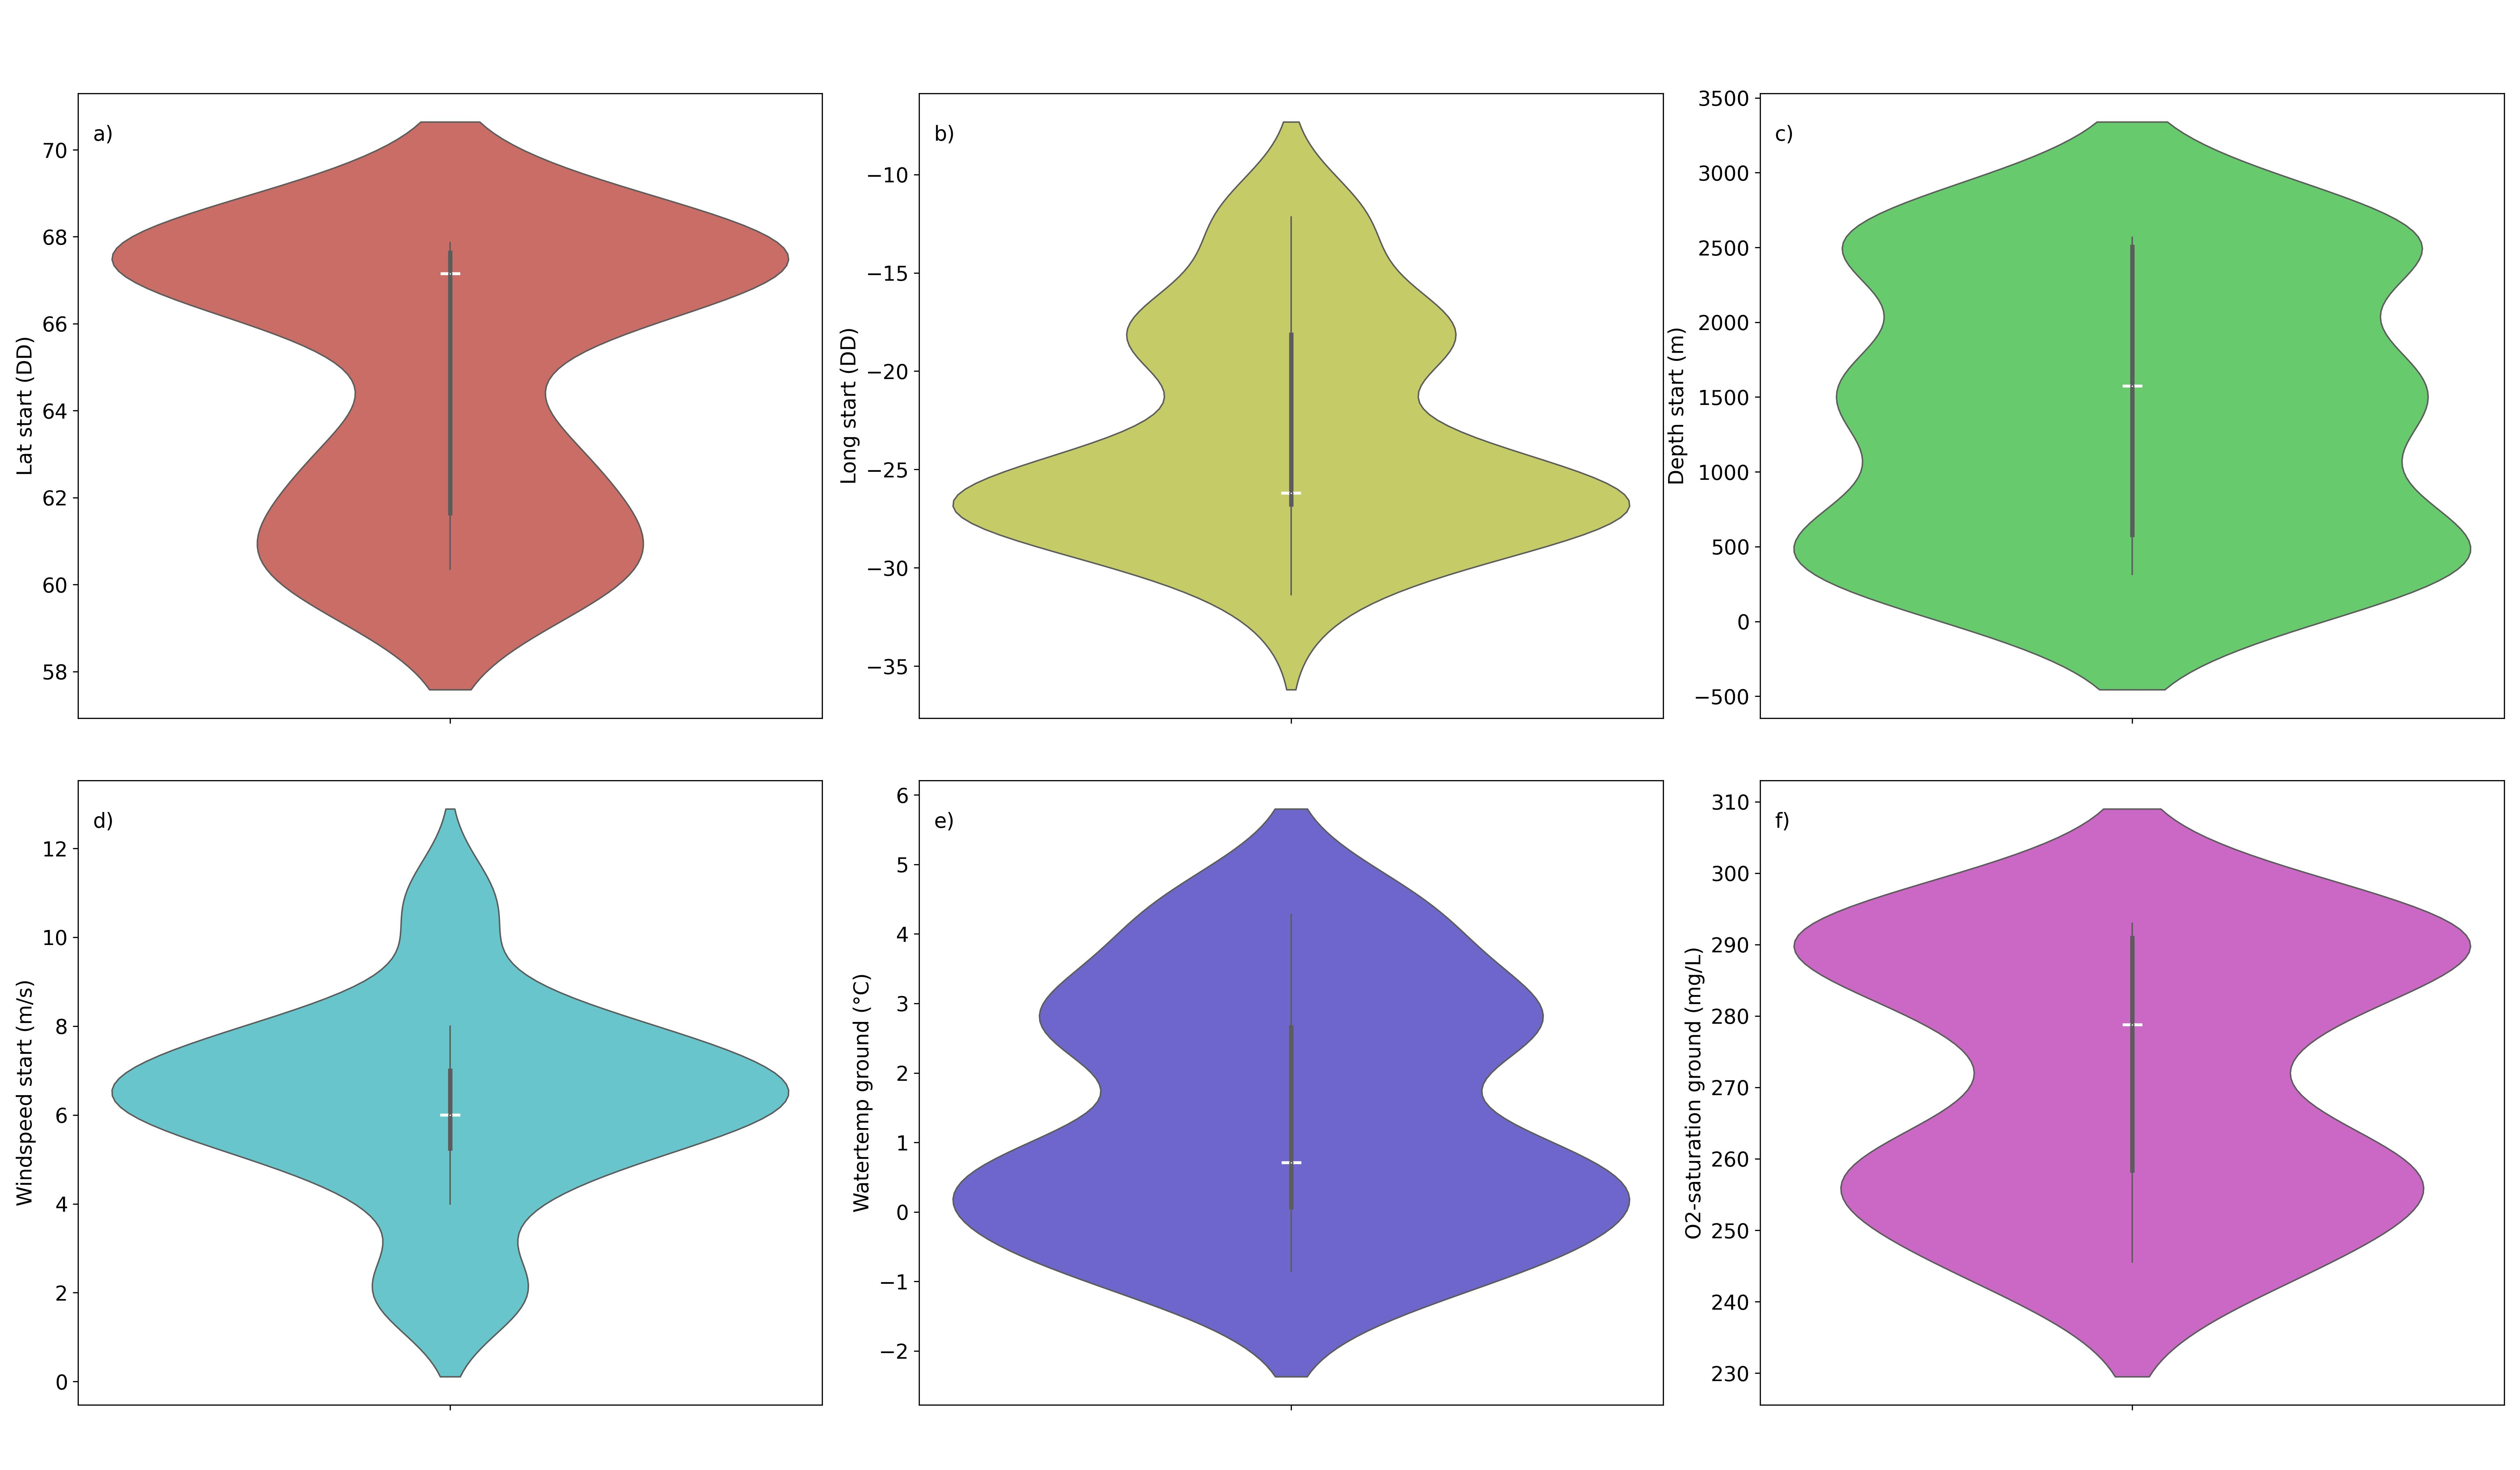
\includegraphics[width=0.7\textwidth]{figure1.jpg}
    \caption{Violin diagrams of six geographic and environmental attributes in our sample. a) Latitude (DD) at the beginning of sampling (red); b) Longitude (DD) at the beginning of sampling (yellow); c) Depth (m) at the start of sampling (green); d) Wind speed (m/s) at the beginning of sampling (light blue); e) Water temperature ($^\circ$C) according to the depth at which the specimens were collected (dark blue); f) O\textsubscript{2} concentration (mg/L) according to the depth at which the specimens were sampled (pink). The mean, median, standard deviation (Std, Dev), 1st quartile (Q1), and 3rd quartile (Q3) of the dataset for each attribute are shown in the top right corner of each chart. \label{fig:fig1}}
\end{figure}

Our results reveal environmental variability in most Cumacea habitats' attributes presented in Figure \ref{fig:fig1} (see supplementary material for a more in-depth analysis). The median of Figure \ref{fig:fig1}a (67.15 DD) is higher than the mean (64.83 DD), indicating a skewed distribution towards lower values. This is also the case for Figures \ref{fig:fig1}c (depth (m)) and \ref{fig:fig1}f (O\textsubscript{2} concentration (mg/L)). The curve of Figure  \ref{fig:fig1}a has a bimodal asymmetric shape, showing two peaks, suggesting that the samples stem from two dominant latitudinal regions at the beginning of sampling. Likewise, this type of curve is present for the longitude (DD) at the start of the sampling as well as for the temperature ($^\circ$C) and O\textsubscript{2} concentration (mg/L) of the water where the samples were collected (see Figures \ref{fig:fig1}b,  \ref{fig:fig1}e and  \ref{fig:fig1}f). 

The median of Figure \ref{fig:fig1}b (-26.21 DD) is lower than the mean (-23.12 DD), indicating an asymmetry on the side of higher values. The standard deviation (5.52 DD) and Quartiles Q1 (-26.77 DD) and Q3 (-18.14 DD) designate a relatively wide range of longitude distribution at the start of sampling (-31.356 - -12.162 DD), suggesting an important geographic distribution and diversity of the samples from east to west in the study region. The standard deviation of Figure \ref{fig:fig1}c is quite high (881.16 m), indicating a vast variability in sample harvesting depths (316 – 2568 m), also supported by Quartiles Q1 (579.10 m) and Q3 (2504.70 m). In contrast to all the other diagrams of Figure \ref{fig:fig1}, the curve in Figure \ref{fig:fig1}c has a multimodal shape with three prominent peaks, suggesting that the samples were collected at various depths, reflecting the diversity of benthic habitats. 

The mean (6.26 m/s) and median (6.00 m/s) of Figure \ref{fig:fig1}d are the only ones in Figure \ref{fig:fig1} that are similar, indicating a symmetrical distribution, with a high concentration of data around the median (6.00 m/s). This suggests relatively stable wind conditions (m/s) at the beginning of sampling. The standard deviation of Figure \ref{fig:fig1}e is relatively high (1.73 °C) compared to the mean (1.45 °C), indicating a broad range of temperatures where samples were taken (0.851 – 4.28 °C). This is also supported by Quartiles Q1 (0.07 °C) and Q3 (2.66 °C). The range of O\textsubscript{2} concentration data (see Figure \ref{fig:fig1}f) shows some variability (245.53 – 292.97 mg/L) as it is presented by the standard deviation (18.11 mg/L) as well as Quartiles Q1 (258.39 mg/L) and Q3 (290.90 mg/L).

\begin{figure}[htbp]
    \centering
    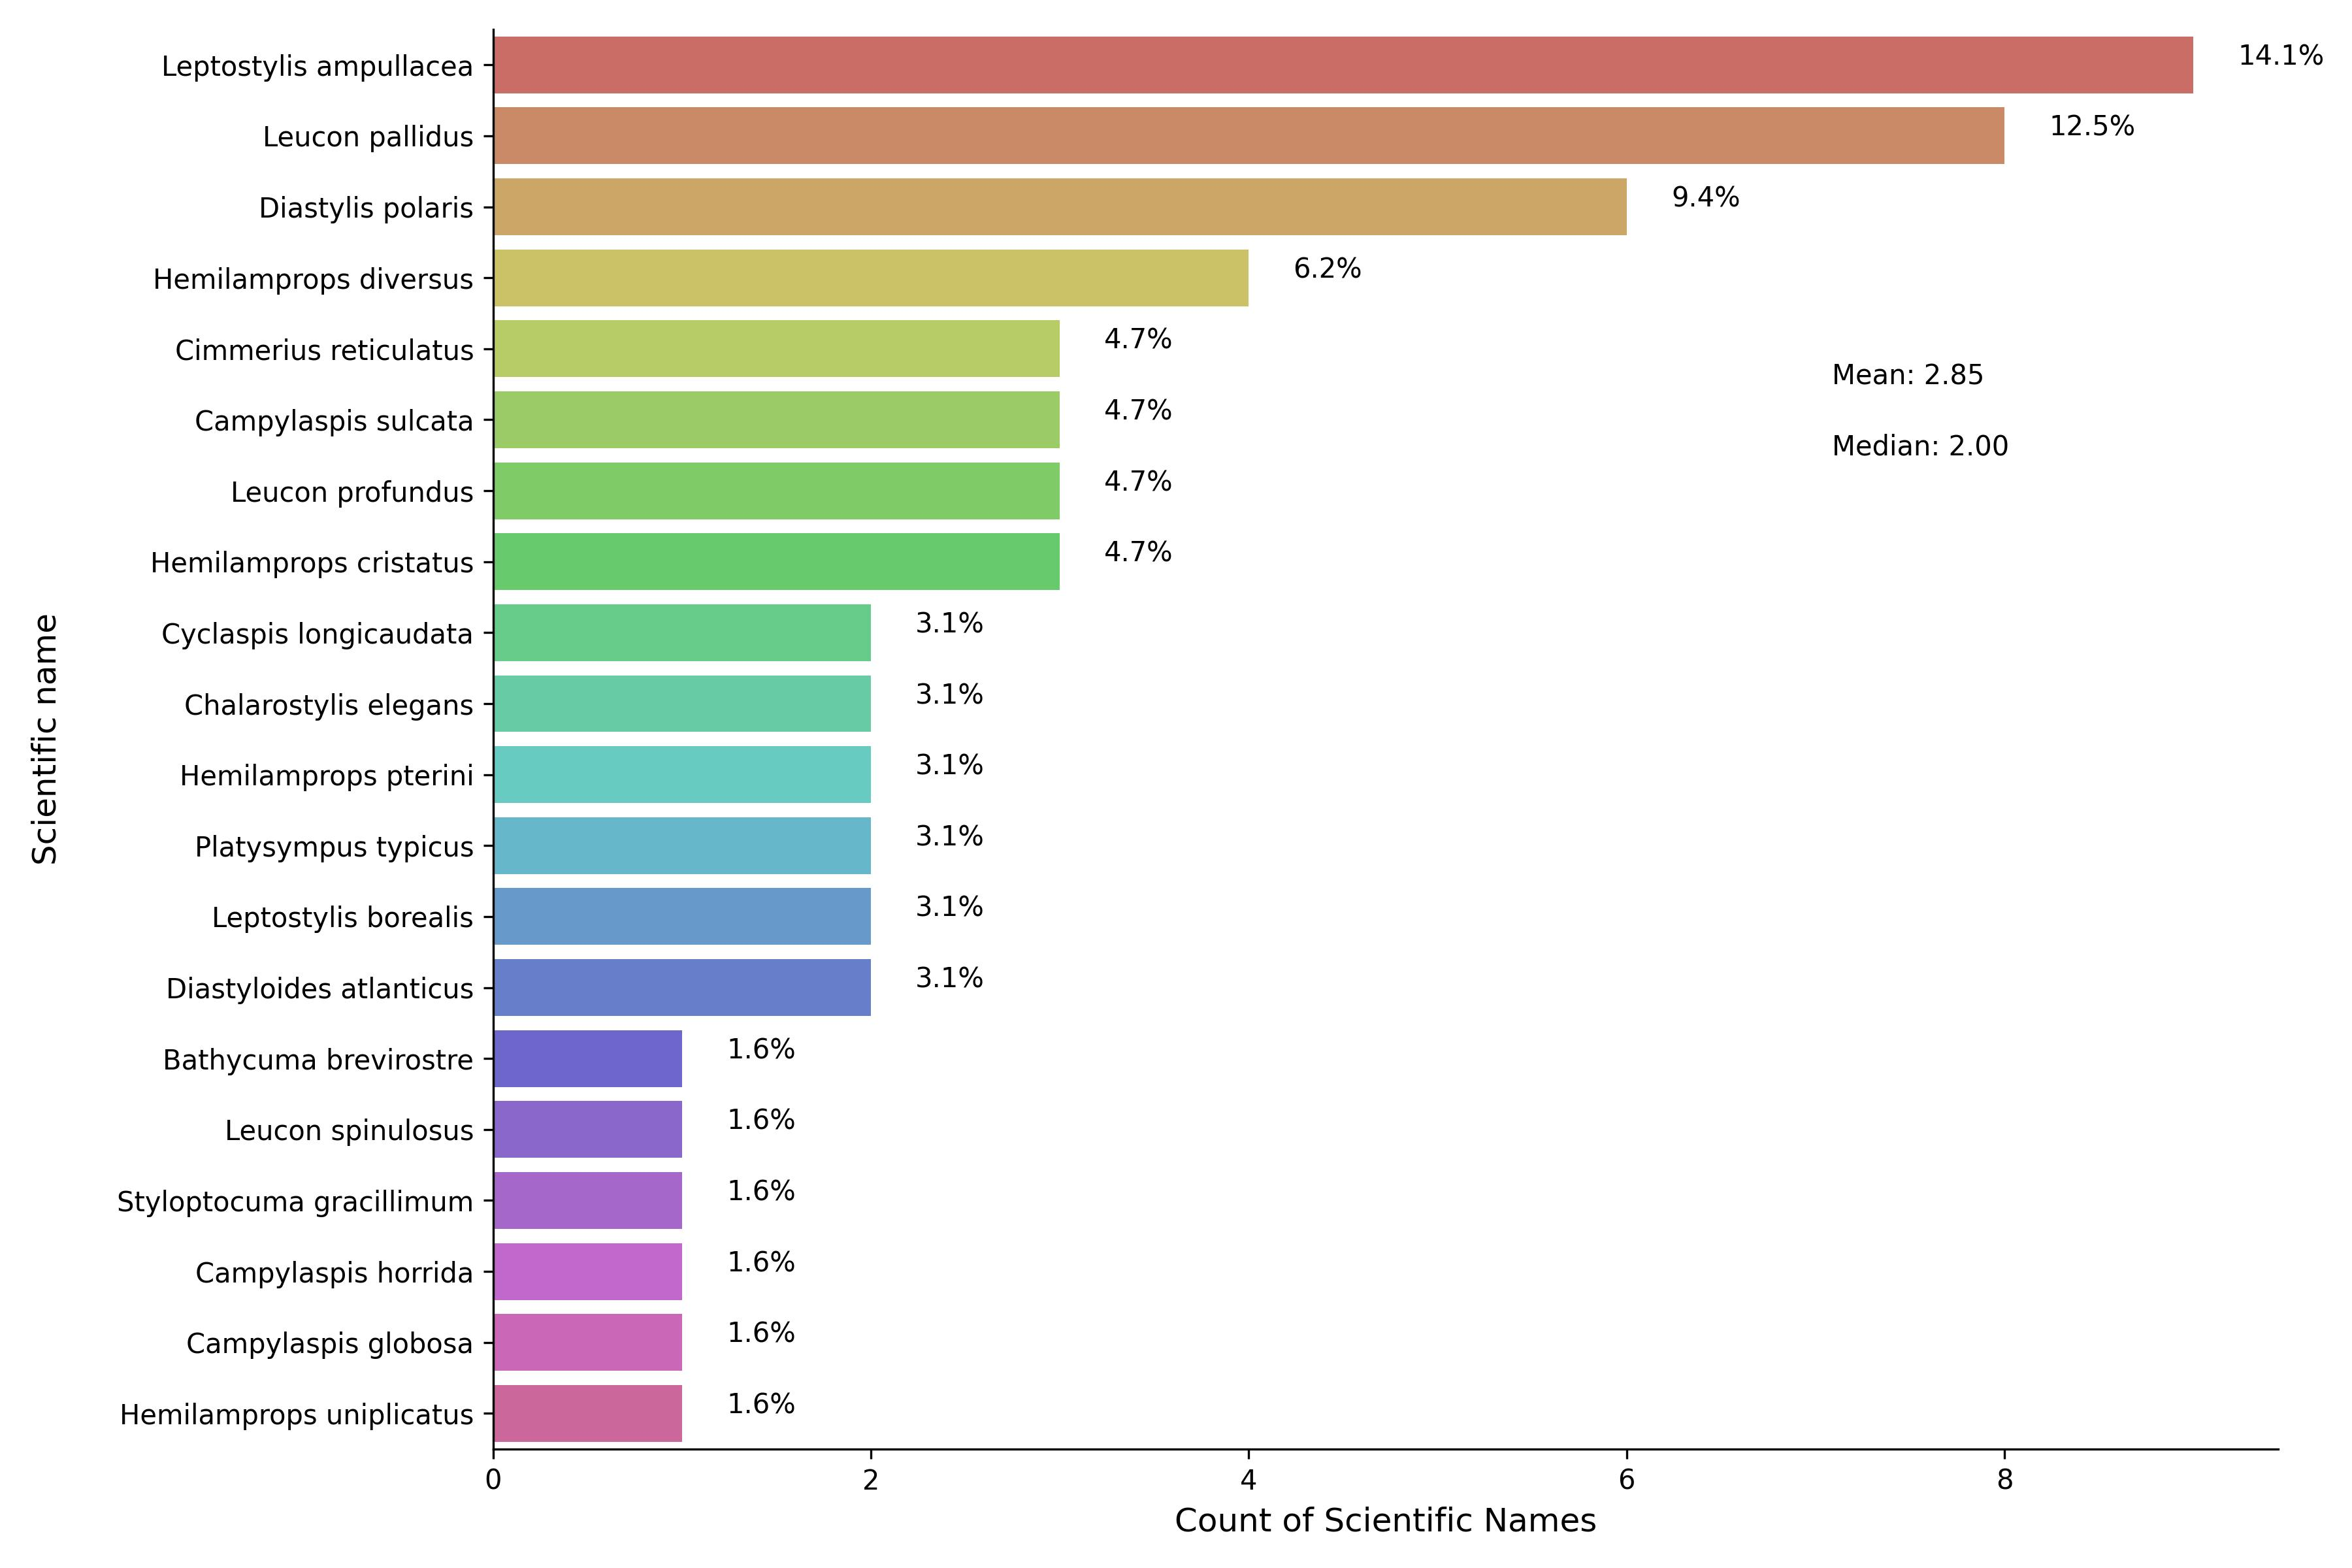
\includegraphics[width=0.7\textwidth]{figure2.jpg}
    \caption{Distribution of Cumacea Species Frequency. This histogram shows the frequency distribution of Cumacea species found in our sample. The bars represent the number of individuals for each species. The percentages displayed above the bars indicate the relative abundance (percentage) of each species within the total sample. The mean and median values of the frequency distribution are presented in the top right corner of the histogram. \label{fig:fig2}}
\end{figure}

The distribution and diversity of the different Cumacea species found in our sample and our analyses are presented in Figure \ref{fig:fig2}. It helps in visualizing the most represented species (\emph{Leptostylis ampullacea}, 14.1\%; \emph{Leucon pallidus}, 12.5\%) and the less represented species (\emph{Bathycuma brevirostre}, \emph{Leucon spinulosus}, \emph{Styloptocuma gracillimum}, \emph{Campylaspis horrida}, \emph{Campylaspis globosa}, and \emph{Hemilamprops uniplicatus}; all 1.6\%), suggesting variations in sampling or particular ecological forces that favor certain species.

\begin{figure}[htbp]
    \centering
    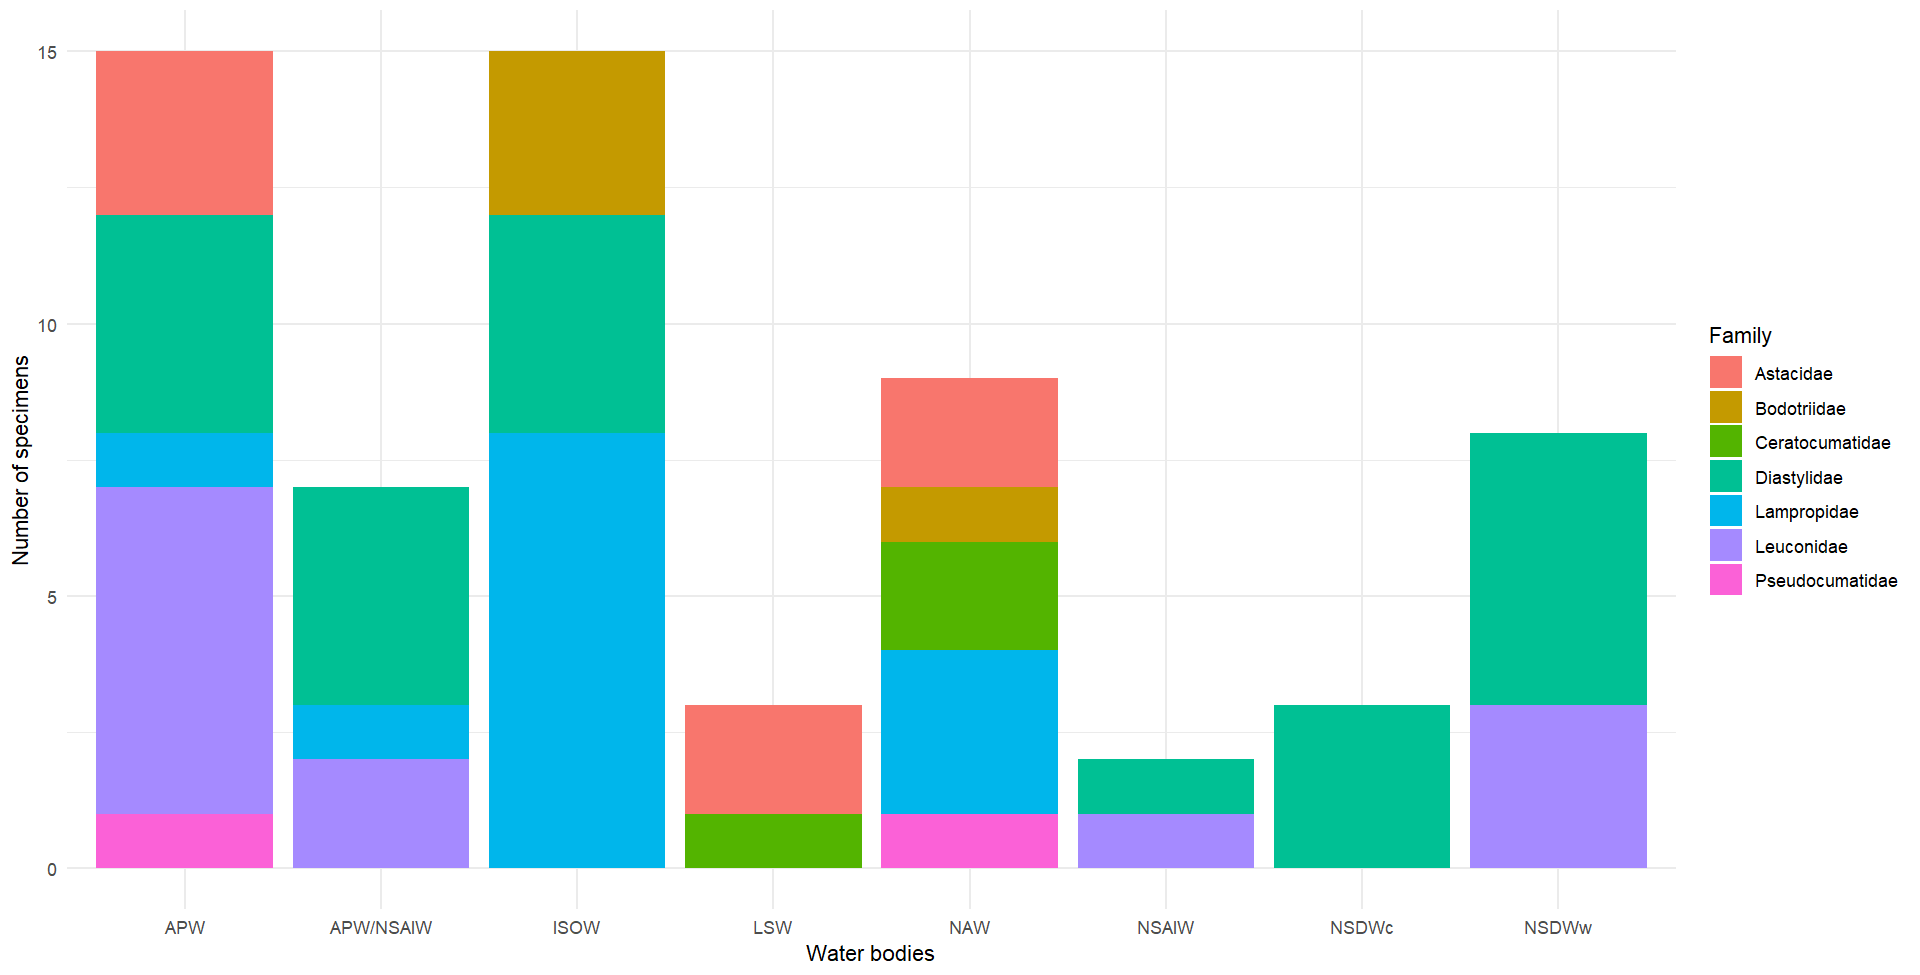
\includegraphics[width=0.7\textwidth]{figure3.png}
    \caption{Distribution of Cumacea Families by Water Body. This histogram depicts the frequency of occurrence for various Cumacea families within our samples, categorized by the water body where they were collected. Eight water body categories are represented: APW (Arctic Polar Water), APW/NSAIW (Arctic Polar Water/North Sub-Arctic Intermediate Water), ISOW (Iceland Scotland Overflow Water), LSW (Labrador Sea Water), NAW (North Atlantic Water), NSAIW  (North Sub-Arctic Intermediate Water), NSDWc (cold North Sub-Atlantic Deep Water), and NSDWw (warm North Sub-Atlantic Deep Water). Seven families are represented: Astracidae (red), Bodotriidae (brown), Ceratocumatidae (green), Diastylidae (turquoise), Lampropidae (blue), Leuconidae (purple), and Pseudocumatidae (pink). \label{fig:fig3}}
\end{figure}

The distribution of samples from different Cumacea families according to the variety of water bodies where they were collected is illustrated in Figure 3. This makes it possible to compare the diversity and potential preferences of the different families in each body of water, with the Diastylidae family being the most present in all the water bodies (turquoise color). In addition, APW and NAW, both of which contain the highest diversity of Cumacea families.

\begin{figure}[]
    \centering
    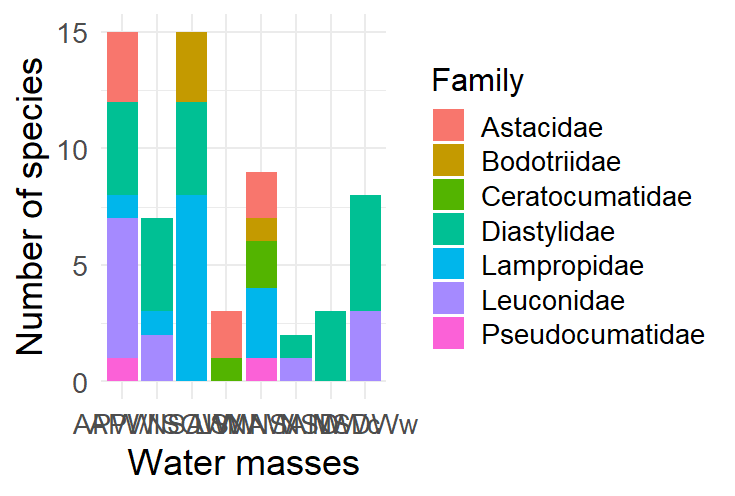
\includegraphics[width=0.7\textwidth]{figure4.png}
    \caption{Distribution of Cumacea Families by habitat. This histogram depicts the frequency of occurrence for various Cumacea families within our samples, categorized by the type of habitat where they were collected. Three habitat categories are represented: Deep sea, Shelf, and Slope. Seven families are represented: Astracidae (red), Bodotriidae (brown), Ceratocumatidae (green), Diastylidae (turquoise), Lampropidae (blue), Leuconidae (purple), and Pseudocumatidae (pink).  \label{fig:fig4}}
\end{figure}

The distribution of samples from different families of Cumacea according to the type of habitat where they were collected during sampling is presented in Figure \ref{fig:fig4}. This makes it possible to compare the diversity of the different families in each type of housing. There is a wide variety of families in the deep sea, mainly dominated by the Diastylidae and the Lampropidae. Shelf also presents a variety of families, but less than the deep sea, with the Leuconidae being the most abundant. Slope, shows the lowest family diversity, with a greater presence of Diastylidae. 


\begin{figure}[]
    \centering
    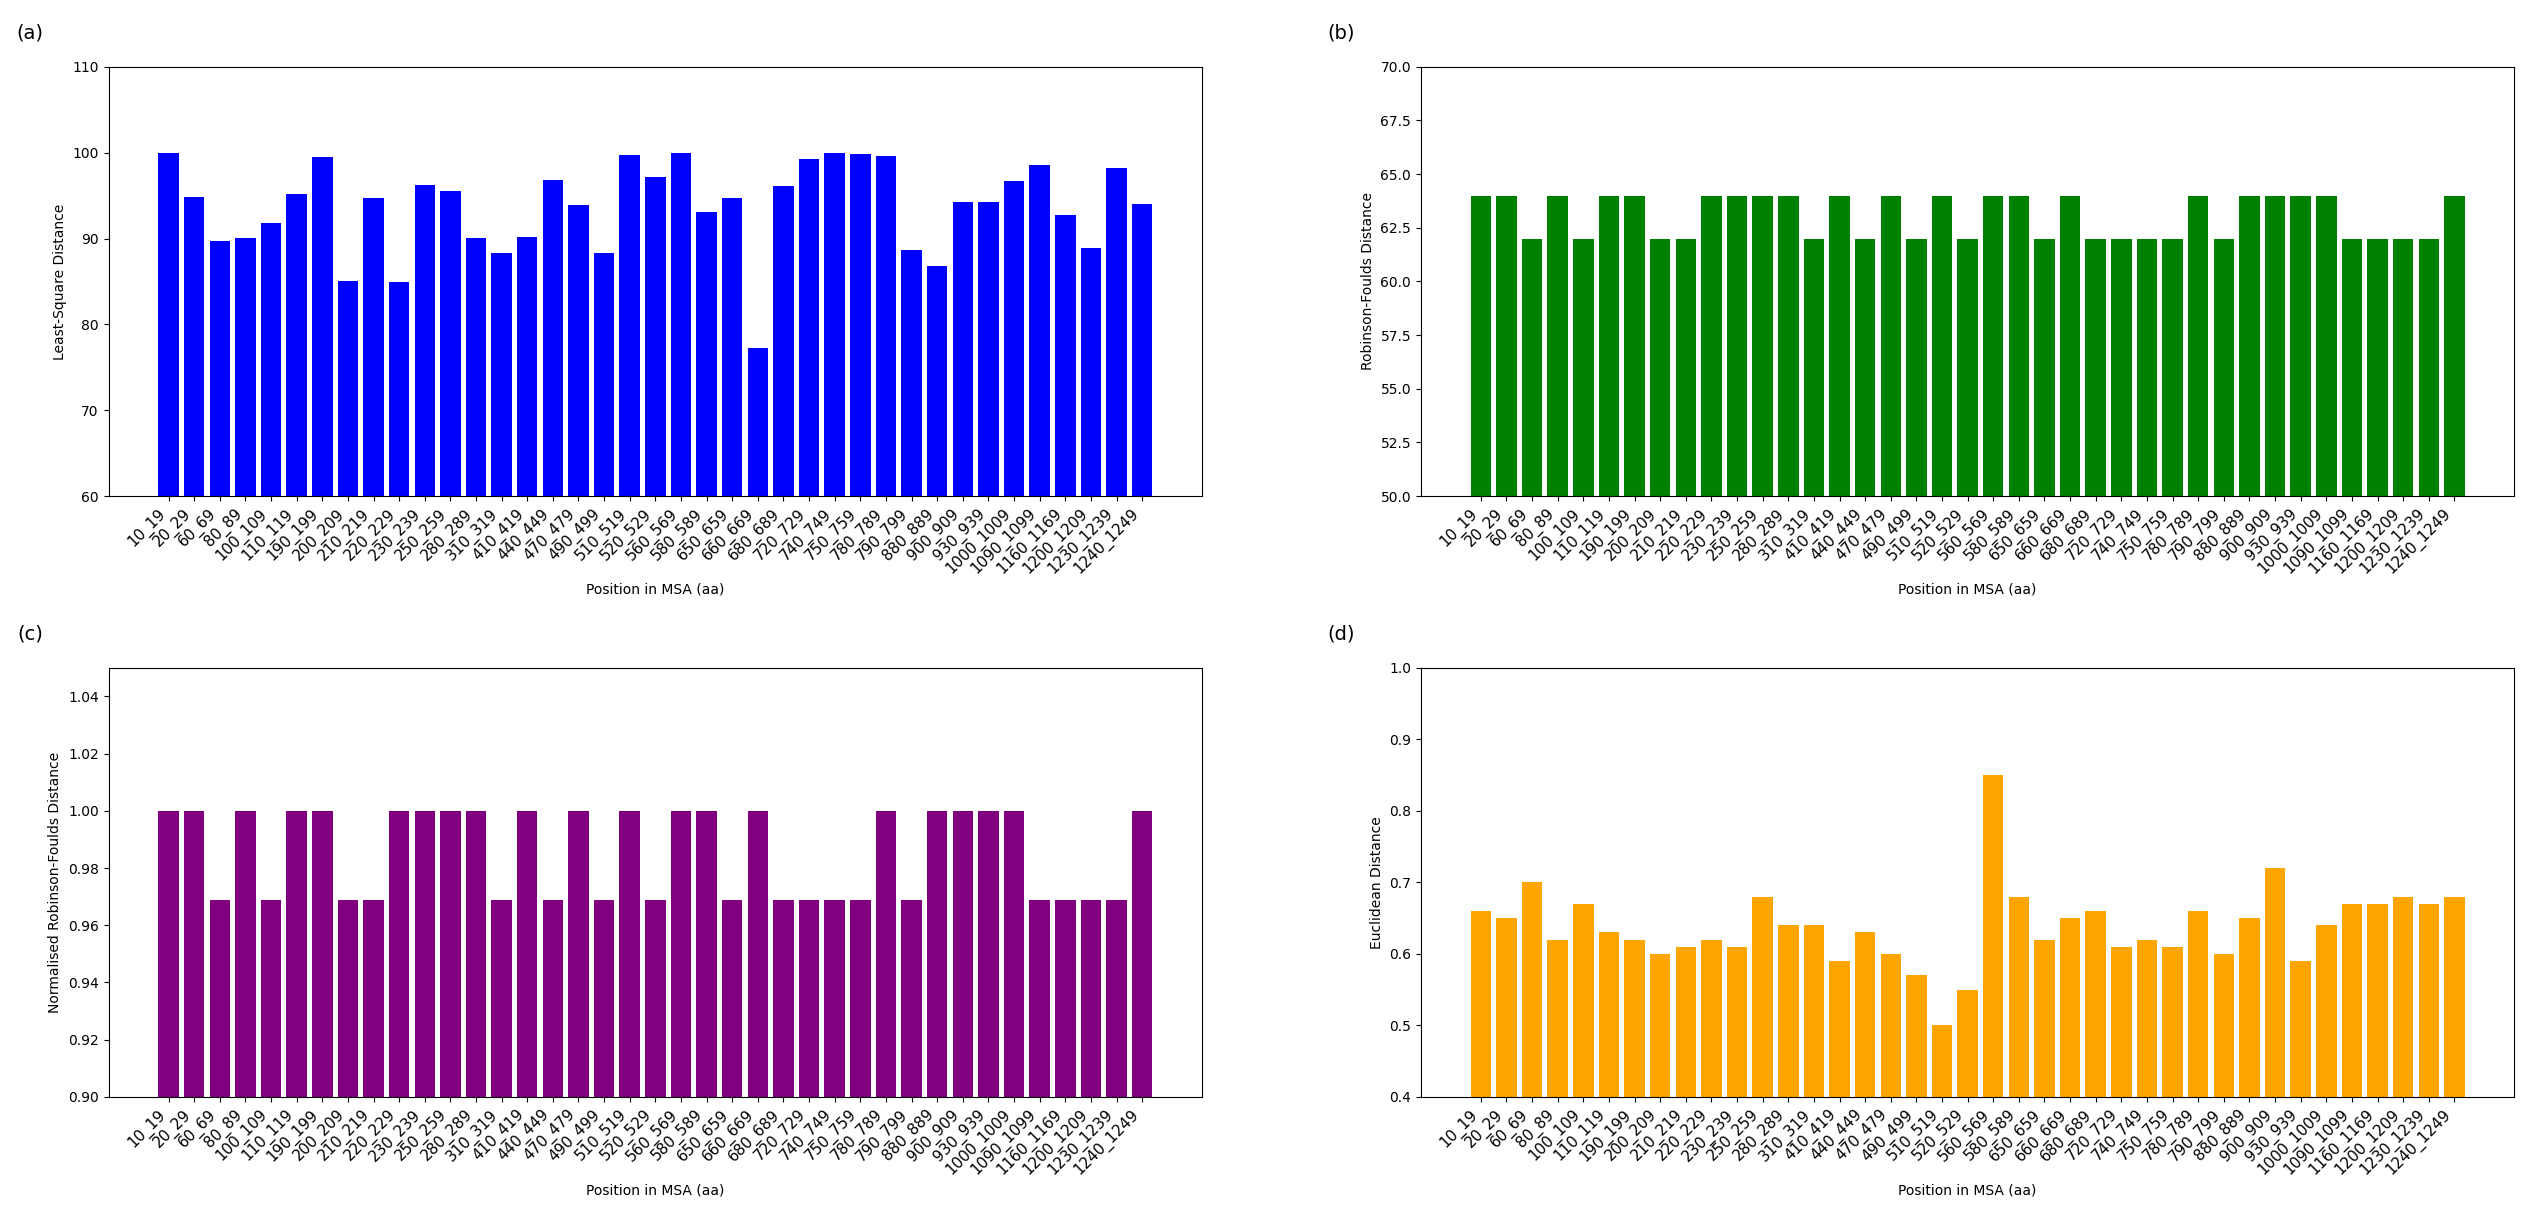
\includegraphics[width=0.7\textwidth]{figure5.png}
    \caption{Analysis of fluctuations in the four distance metrics using multiple sequence alignment (MSA): a) Least-Square distance, b) Robinson-Fouls distance, c) normalised Robinson-Fouls distance, and d) Euclidean distance. These distance variations are studied to establish their correlation with fluctuations in wind speed at the start of sampling (m/s). \label{fig:fig5}}
\end{figure}

\begin{figure}[]
    \centering
    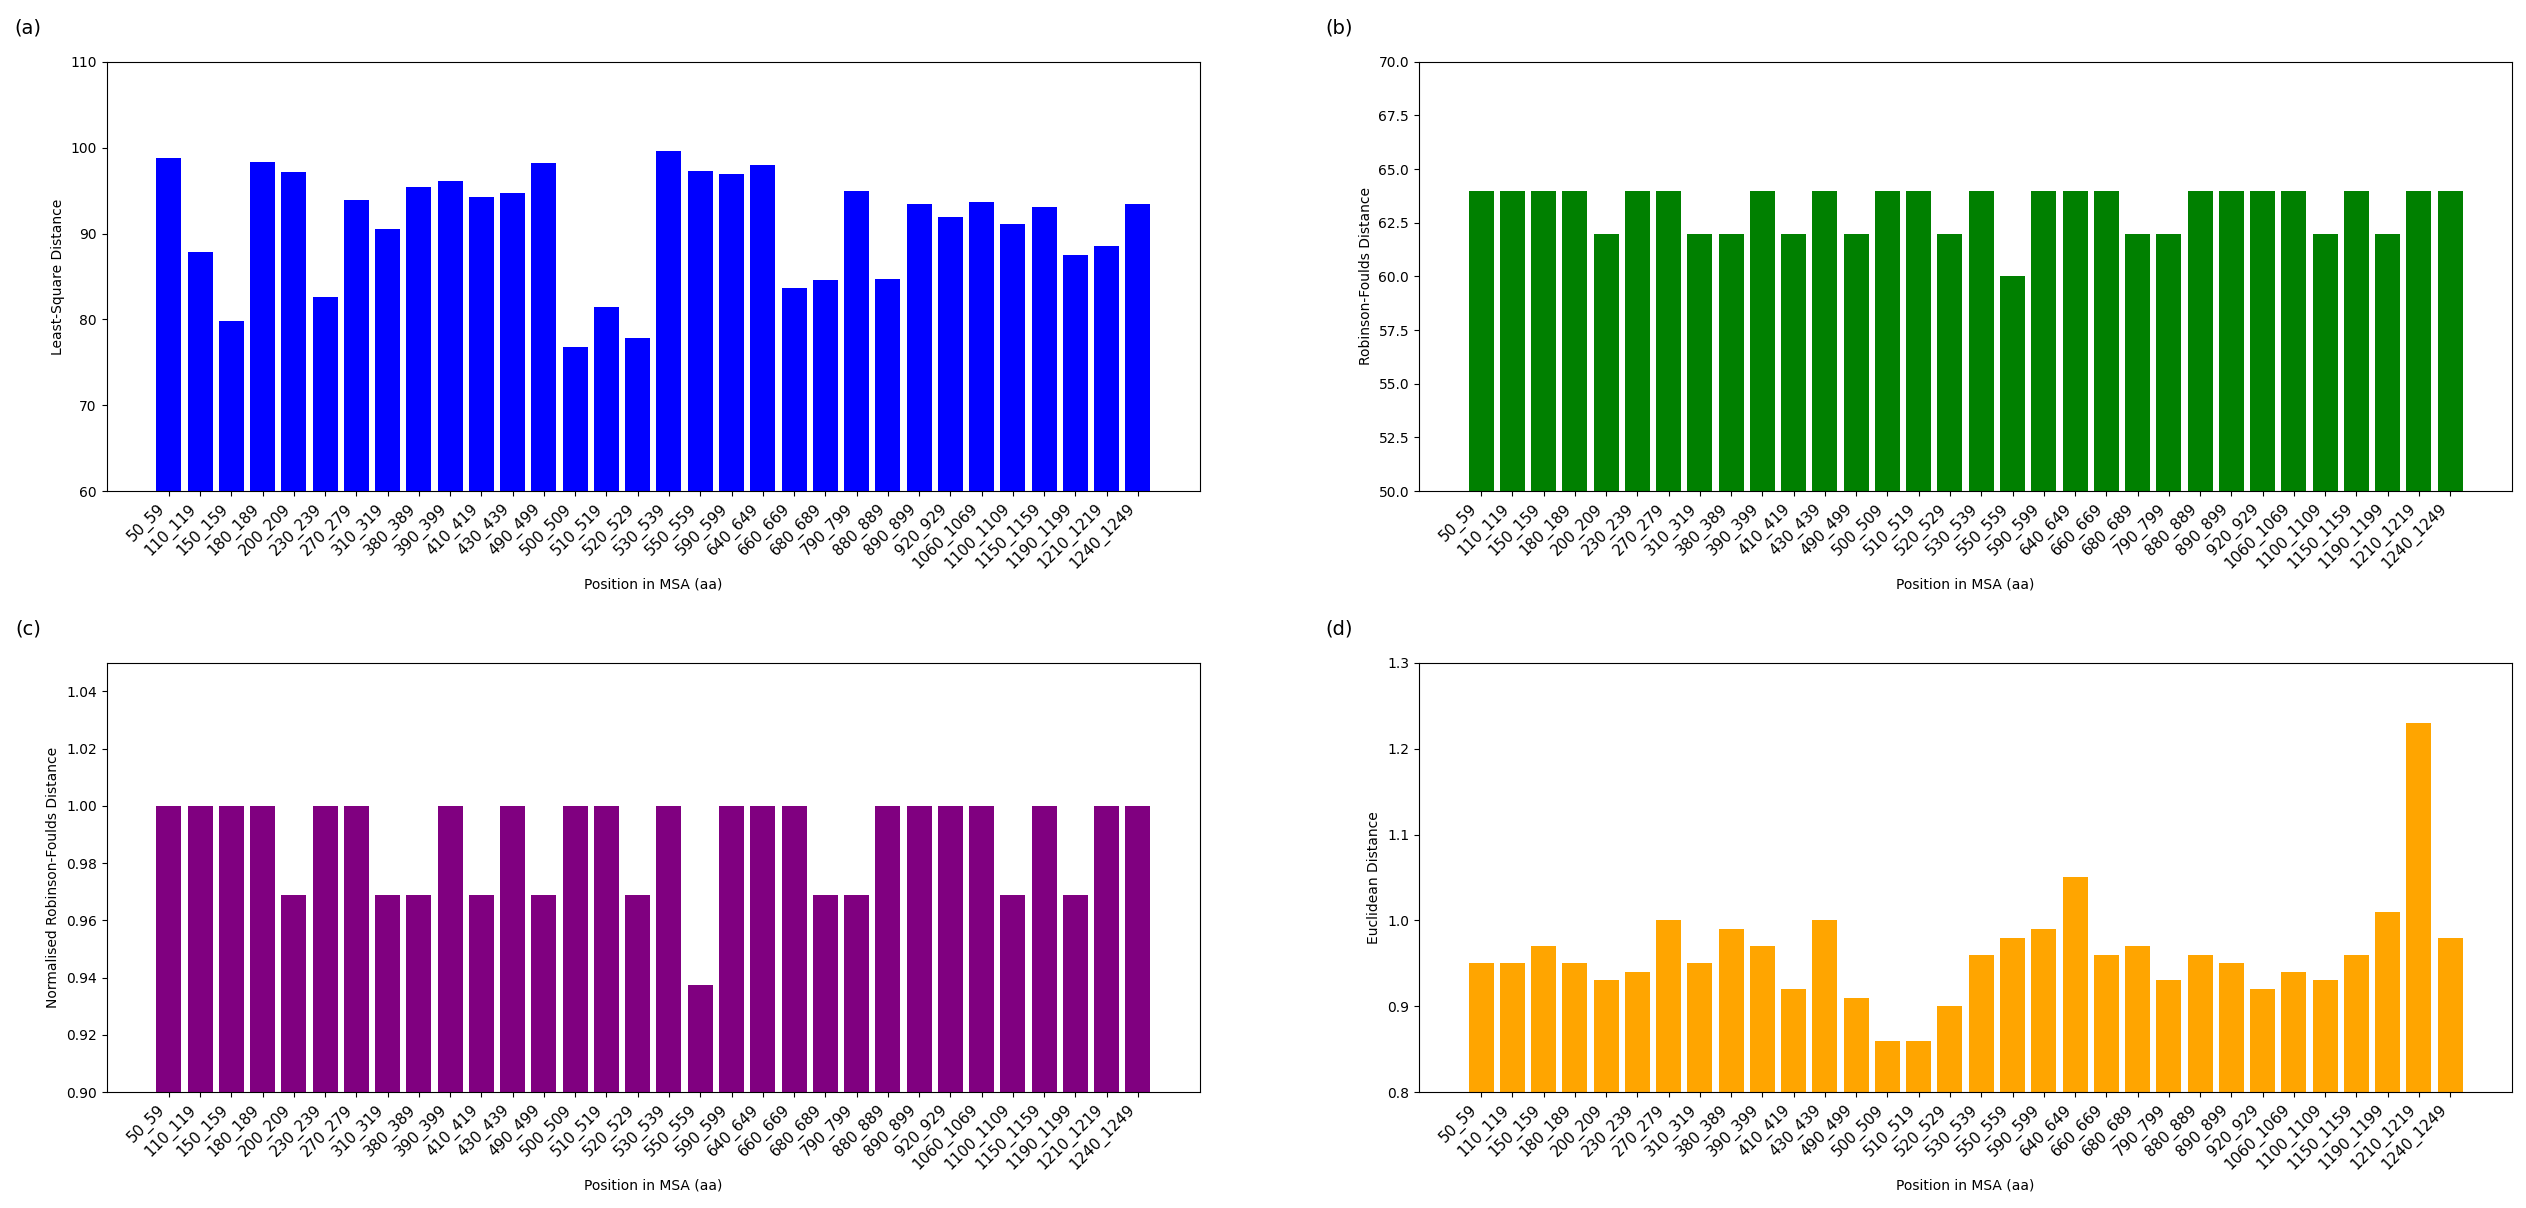
\includegraphics[width=0.7\textwidth]{figure6.png}
    \caption{Analysis of fluctuations in the four distance metrics using multiple sequence alignment (MSA): a) Least-Square distance, b) Robinson-Fouls distance, c) normalised Robinson-Fouls distance, and d) Euclidean distance. These distance variations are studied to establish their correlation with the fluctuation in O\textsubscript{2} concentration where the samples were collected (mg/L). \label{fig:fig6}}
\end{figure}

The correlation between genetic sequences and two attributes, one climatic (wind speed (m/s) at the start of sampling) and the other environmental (O\textsubscript{2} concentration (mg/L)) is presented in Figures  \ref{fig:fig5} and  \ref{fig:fig6}. These correlations are based on four metrics: Least Square Distance, Robinson-Fouls Distance, normalized Robinson-Foulds Distance, and Euclidean Distance. In both Figures, the Euclidean distance appears to be the most sensitive and heterogeneous from our data. A higher Euclidean distance means a greater difference between the sequences at positions 520 to 529 aa (see Figure \ref{fig:fig5}d) and 1190 to 1199 aa (see Figure \ref{fig:fig6}d), suggesting that these sites are more variable or likely to change during evolution.

All these results will need to be further investigated and analyzed to provide a more complete understanding of these results, and thus enable us to draw solid conclusions.

\section{Conclusion}\label{conclusion}

This study focuses on the effect of climatic variables and environmental characteristics on Cumacea (crustaceans: Peracarida) in the waters around Iceland. The main objective is to establish whether there is a correlation between the genetic information of the regions of the 16S rRNA mitochondrial gene (i.e. window) of Cumacea species and the characteristics of their habitats. We wish to determine the environmental attribute most correlated with a specific genetic sequence, as well as the associated protein. We selected relevant attributes from the IceAGE project data, BOLD Systems, and the article by \citep{uhlir_adding_2021}. We eliminated those that were not relevant to this study, as well as those that had low variance (e.g., salinity, $S^2 = 0.02146629$) or abundant missing data (> 95\%). Using these relevant data, we incorporated, in addition to the distribution analyses of certain attributes, phylogeographic studies using the \textit{aPhyloGeo} software (see \autoref{lst:main}). The latter makes it possible to examine potential correlations between the genetics of species and their environment, thus simplifying the interpretation of the evolution of species in various environmental contexts.

The results show significant spatial variability in the Cumacea environment according to two climatic factors, such as the temperature ($^\circ$C) of the water and depth (m) (see Figures \ref{fig:fig1}e and \ref{fig:fig1}c). Excluding wind speed (m/s) at the beginning of sampling, violin diagrams present bimodal or multimodal curves, suggesting geographical and environmental separation of samples. DNA sequence analyses revealed specific genetic windows exposing high mutation rates in response to climatic variables, such as wind speed (m/s) at the start of sampling and water O\textsubscript{2} concentration (mg/L) (see Figures \ref{fig:fig5} and \ref{fig:fig6}). The Euclidean distances of these two parameters showed significant fluctuation across the sequences, indicating sensitive or variable sites in evolution.

The results highlight the importance of understanding the relationships between environmental attributes and genetics of benthic species such as Cumacea. This correlation can be used to explain how these organisms acclimatize to climate change as well as to anthropogenic disturbances, such as seabed mining. These notions are essential for the conservation of deep-sea ecosystems and for predicting the future impacts of environmental fluctuations on marine biodiversity. Our results can highlight conservation plans for regions sensitive to environmental and human disturbance. For instance, the management of fishing and mining activities could use this knowledge to reduce their impact on benthic species. In addition, this research can guide future studies on the genetic adaptation processes of Cumacea to climatic variations.

However, further analysis is needed to examine these results in depth. It is important to note that this study is limited by the number of samples available ($n=62$), the methods used to assess genetic and environmental properties and the logistical burden of data collection. To consolidate these results, it would be pertinent to study other species as well as other geographic regions. In particular, other potentially relevant environmental attributes should be investigated to better interpret genotype-environment interactions.

\section{Acknowledgments}\label{acknowledgments}

The authors thank SciPy conference and reviewers for their valuable comments on this paper as well as Mansour Kebe for his technical support and Carolin Uhlir for her clarifications and advice on her study \citep{uhlir_adding_2021}. This work was supported by the Natural Sciences and Engineering Research Council of Canada (NSERC), the Fonds de recherche du Québec - Nature et technologies (FRQNT), the Université de Sherbrooke grant, and the Centre de recherche en écologie de l’Université de Sherbrooke (CREUS).
